\documentclass{beamer}
\mode<presentation>
\usepackage{amsmath}
\usepackage{amssymb}
%\usepackage{advdate}
\usepackage{adjustbox}
\usepackage{subcaption}
\usepackage{enumitem}
\usepackage{multicol}
\usepackage{mathtools}
\usepackage{listings}
\usepackage{url}
\def\UrlBreaks{\do\/\do-}
\usetheme{metropolis}
\setbeamertemplate{footline}
{
  \leavevmode%
  \hbox{%
  \begin{beamercolorbox}[wd=\paperwidth,ht=2.25ex,dp=1ex,right]{author in head/foot}%
    \insertframenumber{} / \inserttotalframenumber\hspace*{2ex} 
  \end{beamercolorbox}}%
  \vskip0pt%
}
\setbeamertemplate{navigation symbols}{}

\providecommand{\nCr}[2]{\,^{#1}C_{#2}} % nCr
\providecommand{\nPr}[2]{\,^{#1}P_{#2}} % nPr
\providecommand{\mbf}{\mathbf}
\providecommand{\pr}[1]{\ensuremath{\Pr\left(#1\right)}}
\providecommand{\qfunc}[1]{\ensuremath{Q\left(#1\right)}}
\providecommand{\sbrak}[1]{\ensuremath{{}\left[#1\right]}}
\providecommand{\lsbrak}[1]{\ensuremath{{}\left[#1\right.}}
\providecommand{\rsbrak}[1]{\ensuremath{{}\left.#1\right]}}
\providecommand{\brak}[1]{\ensuremath{\left(#1\right)}}
\providecommand{\lbrak}[1]{\ensuremath{\left(#1\right.}}
\providecommand{\rbrak}[1]{\ensuremath{\left.#1\right)}}
\providecommand{\cbrak}[1]{\ensuremath{\left\{#1\right\}}}
\providecommand{\lcbrak}[1]{\ensuremath{\left\{#1\right.}}
\providecommand{\rcbrak}[1]{\ensuremath{\left.#1\right\}}}
\theoremstyle{remark}
\newtheorem{rem}{Remark}
\newcommand{\sgn}{\mathop{\mathrm{sgn}}}
\providecommand{\abs}[1]{\left\vert#1\right\vert}
\providecommand{\res}[1]{\Res\displaylimits_{#1}} 
\providecommand{\norm}[1]{\lVert#1\rVert}
\providecommand{\mtx}[1]{\mathbf{#1}}
\providecommand{\mean}[1]{E\left[ #1 \right]}
\providecommand{\fourier}{\overset{\mathcal{F}}{ \rightleftharpoons}}
%\providecommand{\hilbert}{\overset{\mathcal{H}}{ \rightleftharpoons}}
\providecommand{\system}{\overset{\mathcal{H}}{ \longleftrightarrow}}
	%\newcommand{\solution}[2]{\textbf{Solution:}{#1}}
%\newcommand{\solution}{\noindent \textbf{Solution: }}
\providecommand{\dec}[2]{\ensuremath{\overset{#1}{\underset{#2}{\gtrless}}}}
\newcommand{\myvec}[1]{\ensuremath{\begin{pmatrix}#1\end{pmatrix}}}
\let\vec\mathbf

\lstset{
%language=C,
frame=single, 
breaklines=true,
columns=fullflexible
}

\numberwithin{equation}{section}

\title{Optimization}
\author{Aditya Tripathy\\ Dept. of Electrical Engg.,\\IIT Hyderabad.}

\date{\today} 
\begin{document}

\begin{frame}
\titlepage
\end{frame}

\section*{Outline}
\begin{frame}
\frametitle{Table Of Contents}
\tableofcontents
\end{frame}
\section{Problem}
\begin{frame}
\frametitle{Problem Statement}
%
Find the local minimum/maximum of the given function:\\
$f\brak{x} = x^2$
%A circle $C$ passes through 
%\begin{equation} 
%\vec{P}=\myvec{-2\\ 4} 
%\label{eq:circle_7_p}
%\end{equation} 
%and touches the $y$-axis at 
%\begin{equation} 
%\vec{Q}=\myvec{0\\ 2}. 
%\label{eq:circle_7_q}
%\end{equation}
%Which one of the  following equations can represent a diameter of this circle?
%\begin{enumerate}[label=(\roman*)]
%\begin{multicols}{2}
%\setlength\itemsep{1em}
%\item $\myvec{4 & 5}\vec{x} = 6 $
%\item $\myvec{2 & -3}\vec{x} +10 = 0 $
%\item $\myvec{3 & 4}\vec{x} = 3 $
%\item $\myvec{5 & 2}\vec{x} +4= 0 $
%\end{multicols}
%\end{enumerate}
\end{frame}

%\subsection{Literature}
\section{Gradient Descent}
\subsection{Recursive Formula}
\begin{frame}
    \frametitle{Getting the Difference Equation}
We use the method of gradient descent to find the minimum/maximum of the given function, since the objective function is convex.
Since the coefficient of $x^2 > 0$, we expect to find a local minimum.
\begin{align}
    x_{n+1} &= x_n - \mu f^{\prime}\brak{x_n}\\
    f^{\prime}\brak{x_n} &= 2x_n\\
    \xrightarrow{} x_{n+1} &= x_n - 2\mu x_n \\
    &= \brak{1-2\mu}x_n
\end{align}
%\framesubtitle{Literature}
%Let $\vec{O}$ be the centre of $C$. Then the equation of the normal, OQ is
%\begin{align}
%%\vec{x}^T\vec{x}-2\vec{O}^T\vec{x} +F = 0
%\myvec{0 & 1}\brak{\vec{O}-\vec{Q}} &= 0
%\nonumber \\ 
%\implies \myvec{0 & 1}\vec{O} = 2
%\label{eq:circle_7_o1}
%\end{align}
%%
%Also, 
%%Substituting \eqref{eq:circle_7_p} in \eqref{eq:circle_7_c}, 
%\begin{align}
%\norm{\vec{O}-\vec{P}}^2&=\norm{\vec{O}-\vec{Q}}^2 
%\nonumber \\
%\implies 2\brak{\vec{P}-\vec{Q}}^T\vec{O} &= \norm{\vec{P}}^2-\norm{\vec{Q}}^2 
%\nonumber \\
%\text{or, } \myvec{1 & -1}\vec{O} &= -4
%\label{eq:circle_7_o2}
%\end{align}
%%
%\eqref{eq:circle_7_o1} and \eqref{eq:circle_7_o2} result in the matrix equation
%\begin{align}
%\myvec{1 & -1 \\ 0 & 1}\vec{O} = \myvec{-4\\2}
%\label{eq:circle_7_matrix}
%\end{align}
%yielding the augmented matrix
%\begin{align}
%\myvec{1 & -1 & -4\\ 0 & 1 & 2} \leftrightarrow \myvec{1 & 0 & -2\\ 0 & 1 & 2}\implies \vec{O} = \myvec{-2 \\2}
%\label{eq:circle_7_o}
%\end{align}
%%
\end{frame}
\begin{frame}
\frametitle{Addressing ROC}
Applying unilateral Z-transform,
\begin{align}
    zX\brak{z} - zx_0 &= \brak{1-2\mu}X\brak{z}\\
    \brak{z - \brak{1-2\mu}}X\brak{z} &= zx_0\\
    X\brak{z} &= \frac{zx_0}{z - \brak{1-2\mu}}\\
    X\brak{z} &= \frac{x_0}{1 - \brak{1-2\mu}z^{-1}}\\
    &= \sum_{0}^{\infty} \brak{1-2\mu}^n z^{-n}
\end{align}

%\begin{enumerate}[label=(\roman*)]
%\item $\myvec{4 & 5}\vec{O} = 2 \ne 6 $. Incorrect.
%\vfill
%\item $\myvec{2 & -3}\vec{O} +10 = 0 $. Correct.
%\vfill
%\item $\myvec{3 & 4}\vec{O} = 2 \ne 3 $.  Incorrect.
%\vfill
%\item $\myvec{5 & 2}\vec{O} +4= -2 \ne 0 $. Incorrect
%\end{enumerate}

\end{frame}
\begin{frame}
\frametitle{ROC}
From the last equation, ROC is 
\begin{align}
    |z| &> |1-2\mu|\\
    \xrightarrow{} 1 > |1-2\mu| &> 0\\
    \xrightarrow{} \mu \in \brak{0, 1} \setminus \sbrak{\frac{1}{2}}
\end{align}
Equation 3.11 is due to the following theorem
\end{frame}
\begin{frame}
\frametitle{Theorem}
An LTI system is stable if and only if the ROC of its system function contains the unit circle,
    $\abs{z} = 1$
\end{frame}
\begin{frame}
\frametitle{Finding point of convergence}
Now, if $\mu$ satisfies the previous condition,
\begin{align}
    \lim_{n \to \infty} \norm{x_{n+1} - x_n} = 0\\
    \xrightarrow{} \lim_{n \to \infty} \norm{\brak{-2\mu}x_n} = 0\\
    \xrightarrow{} \norm{\brak{-2\mu}}\lim_{n \to \infty} \norm{x_n} = 0\\
    \xrightarrow{} \lim_{n \to \infty} \norm{x_n} = 0\\
    \xrightarrow{} \lim_{n \to \infty} x_n = 0
\end{align}
\end{frame}
\begin{frame}
\frametitle{Solution}
Taking initial guess = 8\\ step size = 0.01\\ tolerance(minimum value of gradient) = 1e-5\\ We get \\
$x_{min} = 4.910792425174398e-06$\\
\end{frame}

\section{Quadratic Programming}
\begin{frame}
\frametitle{Reformulating}
As a fun exercise, the given question can be posed as the following quadratic programming problem:\\
Find the point lying on the line y = 1, which is nearest to origin.
\\ We can formulate the problem as follows:
\begin{align}
    \min_{\vec{x}} \norm{e_2^{\top}\vec{x}}^2\\
    \text{s.t. } \\ \vec{x}^{\top}V\vec{x} + 2\vec{u}^{\top}\vec{x} + f = 0\\
    V = \myvec{1 & 0 \\ 0 & 0}\\
    \vec{u} = \myvec{0 \\ -0.5}\\
    f = 0\\
\end{align}
\end{frame}
\begin{frame}
\frametitle{Relaxation of Constraint}

In the current form, the constraint is non-convex since the constraint defines a set which is not convex, since points on the
line joining any 2 points on the curve don't belong to the set. However, if we become lenient and make the constraint
\begin{align}
    \vec{x}^{\top}V\vec{x} + 2\vec{u}^{\top}\vec{x} \le 0
\end{align}
the constraint becomes convex. Using cvxpy to solve this convex optimization problem, we get \\
\begin{align}
    Optimal x: [[0.00000000e+00]\\
 [8.63053066e-11]]
\end{align}
\end{frame}
%\section{Plot}
\subsection{Graph}
\begin{frame}[fragile]
\frametitle{Graph}
\begin{figure}[h!]
   \centering
   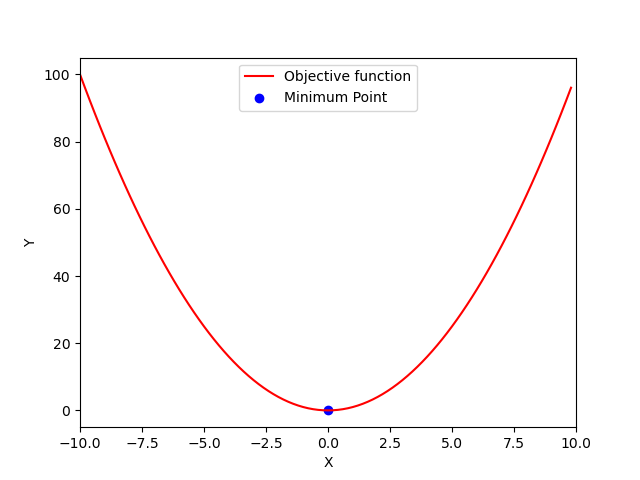
\includegraphics[width=0.7\linewidth]{figs/fig.png}
   \caption{Minimum Value of Objective function}
\end{figure}
\end{frame}
\end{document}
